\chapter{Preliminaries}

In this chapter design requirements for the robot will be determined based on minimal required capabilities. 
Followed by an evaluation of stepper motor based locomotion for a transiently powered robot.

\section{Design Requirements}
\label{sec:design_requirements}

% RF harvesting seems prommesing
% Wispcam requires approx 4 seconds to harvest 20mJ at a distance of 20cm from the reader \cite{naderiparizi_rfid_2015}
% better to only use RF for communication and harvest energy from another source \cite{konstantioulos}

% Energy can be harvested from different sources


% - Small form factor
% - Weight of the robot
% - Power (should not rely on batteries)
% - Low voltage decreases power consumption of components and allows efficient use of the energy from the supercapacitor

% - Optimize or low power consumption (disable or standby sensors and motor ctrl when not used)
% - Minimal basic functionality (for simple swarm algorithms?) (but no power hungry components ie optical encoders or mouse sensors)
% - Low power communication
% - Navigation

Furthermore:
% - Single mainboard design
% - Off the chelf components
% - Swarm robots are typically limited to only operate on flat surfaces!
% - However should be able to be powered from batteries for testing and tuning!

% Extra extra:
% - Tradeoff chargetime and operation time


Current state of the art micro robotic platforms are not bigger than 4.4 cm, as can be seen from Table \label{tab:comparison_robot_platforms}.
Keeping the size of the robot to a minimum is beneficial, while the weight will scale accordingly and less energy will be required for movement.



Typically the amount of power that can be harvested 

The main requirement for the robot is that it should be battery-less, therefore it can only store a small amount of energy in a capacitor / small buffer.
The leakage current increases with the capacitance of the capacitor and the voltage stored in the capacitor.
As a result these require longer charge time

To make efficient use of the energy stored in a supercapacitor a regular is required to supply a stable voltage to the connected loads.
The regulated output voltage is a lower threshold for the energy that can be used from the capacitor.
The upper threshold is typically determined by the maximum voltage rating of the supercapacitor.
Lowering the output voltage allows for more energy to be used from the supercapacitor, but also lowers the overall power consumption of individual components.
The energy stored in supercapacitor is a function of the capacitance and the threshold voltage difference, being equal to:

\begin{equation}
\label{eq:cap2}
E = \frac{1}{2}C(V_{\max} - V_{\min})^{2}
\end{equation}

\section{Stepper motor-based Locomotion}

One of the major requirements for the robot was that it should have accurate locomotion and basic odometry.
Wheel encoders are typically used to estimate the angular speed of the wheels.
A combination of LEDs and photo diodes are used to measure the reflection of a rotating disk.
However, two LED's on constantly on could consume a lot of power relative to the power budget of the transiently powered robot.
The GRITSBot uses stepper motors to achieve accurate locomotion and basic odometry, as described in Section \ref{sec:locomotion}.
This section will further investigate the use of stepper motor based locomotion in combination with a transiently-powered robot.

\subsection{The stepper motor}
A stepper motor is a type of permanent magnet dc motor that starts to rotate by supplying current to the motor coils in a specific direction.
The bipolar stepper motor used, requires current to be pulsed trough each of the four connections, in a fixed pattern, in order to rotate it forward or backward.
A Microcontroller (MCU) is used to keep track and instruct the next stepper motor position from a sequence of four.
The outputs of the MCU cannot supply enough current to drive a bipolar stepper motor, therefore a dual H-bridge is required to control the current trough each coil.

\begin{figure}
	\centering
	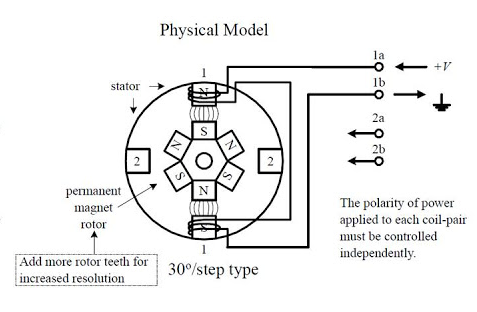
\includegraphics[width=\textwidth]{pics/bipolar_stepper.png}
	\caption{http://homemaderobo.blogspot.nl/2012/03/stepper-motor.html}
	\label{fig:bipolarstepper}
\end{figure}

The only way to grantee that the teeth on the rotor will stay aligned with the coil is to keep the coil energized until the next position is instructed and the other coil is energized. 
On the first startup it can happen that the rotor is not aligned with the last position in the sequence.
When this happens there can be an error between one and three steps of instructing a new steps and the stepper moving to the next position.

In case the stepper motor is rotating and the power is removed, misalignment between the rotor and the last energized coil can occur.
While the rotor could be moving from one position to the next, it has not moved at all (undershoot) or it overshoots it's next position due to inertia of the rotating mass. 
To determine what would be more likely, undershooting or overshooting, an experiment has been preformed to determine the error in number of steps.

A stepper motor is suspended and a needle glued to the motor shaft.
The needle rotates over a round piece of paper which is divided by markings every 18 degrees, as can be seen from Figure \ref{fig:step_counting}.
First the rotor and coil is synchronized by moving 4 steps.
Then the position of the needle is recorded and the stepper motor is commanded to make one rotation equal to 20 steps.
After rotating 20 steps the power is removed and the needle position recorded when the needle is not rotating anymore.

\begin{figure}
	\centering
	\begin{subfigure}[b]{0.38\textwidth}
		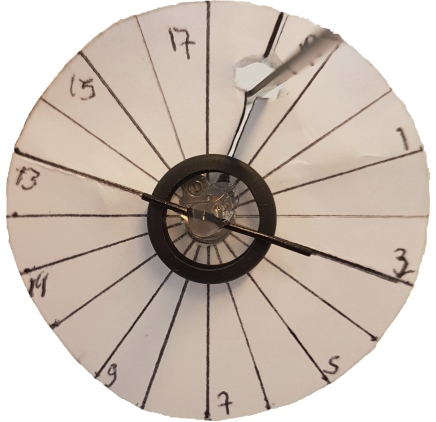
\includegraphics[width=\textwidth]{pics/step_counting.jpg}
		\caption{Experimental setup for determining error in the number of counted steps}
		\label{fig:step_counting}
	\end{subfigure}
	\quad
	\begin{subfigure}[b]{0.55\textwidth}
		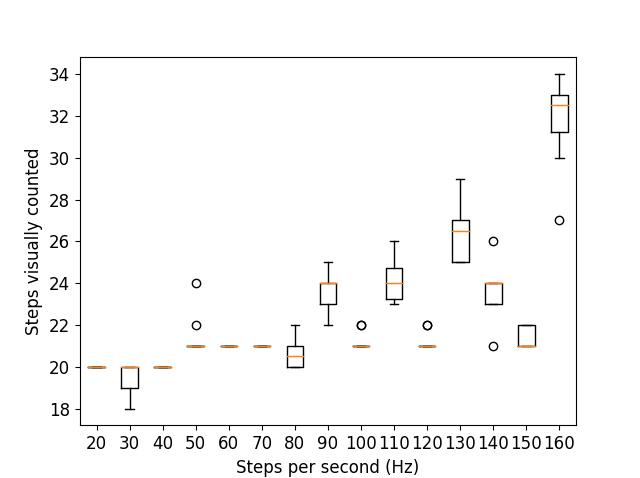
\includegraphics[width=\textwidth]{pics/figure_intertia.png}
		\caption{}
		\label{fig:step_results}
	\end{subfigure}
	\caption{}
\end{figure}

\subsection{Result}

% Differential drive robot using two stepper motors has a 

%The current trough the coils is constant, so the faster the stepper motor changes step the more energy can be transformed into movement.
%Increasing the rotational speed of the stepper motor decreases the torque output of the motor.
%Therefore the speed is limited by the amount of torque required to preform the movement.





